\chapter{Outils, Méthodologies et Architecture}
\label{chap:Chapter 3 title}
\section*{Introduction}

\hspace{\parindent}Le chapitre "Outils, Méthodologies et Architecture" revêt une importance capitale dans la contextualisation de notre projet. Il offre une vue d'ensemble précieuse sur les environnements technologiques dans lequel notre projet évolue, ainsi que sur les outils et les ressources nécessaires à sa réalisation.

Dans ce chapitre, nous détaillons les différents composants qui constituent notre environnement de développement et de test. Nous mettons en lumière les langages de programmation utilisés, les frameworks et les bibliothèques mobilisés, ainsi que les exigences matérielles et logicielles spécifiques au projet. De plus, nous abordons les méthodologies de travail et les concepts fondamentaux qui guident notre approche.

Cette connaissance approfondie de notre environnement et des outils disponibles nous a permis de prendre des décisions éclairées tout au long du processus de développement. Elle a également été cruciale pour optimiser notre architecture, garantissant ainsi la mise en place d'une solution robuste et efficace.

\newpage


\section{Langages de programmation}

\hspace{\parindent}Dans cette section, nous abordons les langages de programmation essentiels à notre projet, mettant en lumière leur rôle central dans le processus de développement. Nous nous concentrons sur l'importance de choisir des langages compatibles et cohérents pour garantir l'efficacité et la fluidité de notre travail tout au long du cycle de développement.

\textbf{C\#} : est un langage de programmation orienté objet et orienté composant. Ses structures de langage intègrent directement ces concepts, ce qui en fait un choix naturel pour la création et l'utilisation de composants logiciels. Depuis ses débuts, C\# a continué à évoluer en ajoutant des fonctionnalités pour répondre à de nouveaux cas d'utilisation et aux pratiques émergentes en conception logicielle. Ce choix est motivé par la robustesse, la clarté et la polyvalence de C\#, ainsi que par son intégration étroite avec la plateforme .NET. En utilisant C\#, nous bénéficions d'un langage moderne et éprouvé qui offre une grande productivité aux développeurs, une facilité de maintenance du code et une compatibilité avec un large éventail de technologies et de frameworks.
\\
\begin{figure}[H] 
    \centering
    
\includegraphics[width=4cm]{Figures/csharp.png}
    \caption{C\#}
    %\label{fig:my_label} %Optional (If you want to reference the figure in later chapters)
\end{figure}


\textbf{SQL}, ou Structured Query Language, est un langage de programmation crucial pour interagir avec les bases de données. Il constitue un outil fondamental pour les développeurs web, leur permettant de gérer et de manipuler efficacement les données stockées dans les sites internet.
\\
\begin{figure}[H] 
    \centering
    
\includegraphics[width=6cm]{Figures/sql.png}
    \caption{SQL}
    %\label{fig:my_label} %Optional (If you want to reference the figure in later chapters)
\end{figure}



\textbf{JavaScript} est utilisé de manière significative pour le développement d'applications web interactives. Nous l'utilisons pour améliorer l'expérience utilisateur en ajoutant des fonctionnalités dynamiques telles que des animations, des validations de formulaire en temps réel et des mises à jour de contenu sans rechargement de la page. De plus, JavaScript est utilisé pour intégrer des frameworks et des bibliothèques frontend populaires tels que React.js ou Angular.js, qui offrent des fonctionnalités avancées pour la création d'interfaces utilisateur réactives et complexes. En outre, JavaScript est également employé côté serveur avec Node.js pour gérer des tâches backend telles que la manipulation de
\\
\begin{figure}[H] 
    \centering
    
\includegraphics[width=5cm]{Figures/javascript.png}
    \caption{JavaScript}
    %\label{fig:my_label} %Optional (If you want to reference the figure in later chapters)
\end{figure}






\section{Framework et bibliothèques}

\hspace{\parindent}Nous examinons les frameworks et les bibliothèques qui ont simplifié le développement de notre projet, en présentant les outils et les ressources qui contribuent à accroître notre efficacité et notre productivité. Nous mettons en lumière les avantages et les fonctionnalités de ces frameworks, qui joueront un rôle crucial dans la réalisation efficace de notre projet.

\textbf{Angular} : est un framework JavaScript développé par Google, largement reconnu pour sa capacité à créer des applications web dynamiques et interactives. Grâce à son architecture modulaire, Angular simplifie la gestion et la maintenance des grandes applications en les divisant en modules fonctionnels distincts. Cette approche organisée permet de rendre le code plus évolutif et facilite la collaboration entre les membres de l'équipe de développement. De plus, Angular offre un système de gestion de l'état robuste, assurant une synchronisation efficace entre les composants de l'interface utilisateur et les données du backend. Cette synchronisation cohérente des données contribue à offrir une expérience utilisateur fluide et réactive, même pour des applications complexes. Enfin, grâce à son moteur de rendu rapide et à sa gestion efficace de la mémoire, Angular garantit des performances optimales, ce qui est essentiel pour fournir une expérience utilisateur de haute qualité.
\\
\begin{figure}[H] 
    \centering
    
\includegraphics[width=6cm]{Figures/angular.png}
    \caption{Angular framework}
    %\label{fig:my_label} %Optional (If you want to reference the figure in later chapters)
\end{figure}



\textbf{Node.js} : est un environnement d'exécution JavaScript côté serveur, basé sur le moteur JavaScript V8 de Google Chrome. Contrairement à d'autres environnements d'exécution JavaScript, Node.js permet d'exécuter du code JavaScript côté serveur, ce qui ouvre de nouvelles possibilités pour le développement d'applications web. Grâce à sa nature asynchrone et non bloquante, Node.js est particulièrement efficace pour gérer de nombreuses connexions simultanées, ce qui en fait un choix idéal pour les applications en temps réel telles que les applications de chat ou les tableaux de bord de données en temps réel. De plus, Node.js dispose d'un vaste écosystème de packages et de modules, disponibles via le gestionnaire de packages npm, ce qui facilite le développement et l'intégration de nouvelles fonctionnalités dans les applications. En outre, Node.js est extensible et peut être utilisé pour créer des applications web, des API RESTful, des applications de streaming, des outils en ligne de commande et bien plus encore. En résumé, Node.js est un outil puissant et polyvalent pour le développement d'applications côté serveur, offrant une performance élevée, une évolutivité et une flexibilité.
\\
\begin{figure}[H] 
    \centering
    
\includegraphics[width=6cm]{Figures/nodejs.png}
        \caption{Node JS logo}
    %\label{fig:my_label} %Optional (If you want to reference the figure in later chapters)
\end{figure}






\textbf{ABP Framework (version 6.0)} : Le choix de ABP Framework (version 6.0) pour notre projet repose sur une série de facteurs clés qui garantissent la pertinence et l'efficacité de notre approche de développement.

ABP Framework est un cadre de développement open source conçu pour faciliter la création rapide et efficace d'applications web et mobiles modernes. Il offre une architecture solide et modulaire, ainsi qu'une multitude de fonctionnalités prêtes à l'emploi, permettant ainsi aux développeurs de se concentrer sur la logique métier de leurs applications plutôt que sur les aspects techniques.

Ce framework prend en charge plusieurs langages de programmation, notamment C\# pour le backend et TypeScript pour le frontend, offrant ainsi une flexibilité et une compatibilité avec les technologies modernes. De plus, ABP Framework intègre des bibliothèques populaires telles que Entity Framework Core pour la gestion des bases de données et Angular pour le développement de l'interface utilisateur, ce qui garantit la robustesse et la pérennité de notre solution.

L'un des avantages majeurs d'ABP Framework est sa capacité à fournir des modules prédéfinis, tels que Identity Server, qui simplifient le développement d'aspects critiques tels que l'authentification et l'autorisation. Cette approche modulaire et extensible permet aux développeurs de personnaliser facilement leurs applications en fonction de leurs besoins spécifiques, tout en bénéficiant d'une base solide et sécurisée.

Le choix d'ABP Framework pour notre projet s'inscrit dans une stratégie visant à optimiser le processus de développement, à garantir la qualité et la sécurité de notre solution, et à assurer sa pérennité à long terme
\\
\begin{figure}[H] 
    \centering
    
\includegraphics[width=8cm]{Figures/abp.png}
        \caption{ABP framework logo}
    %\label{fig:my_label} %Optional (If you want to reference the figure in later chapters)
\end{figure}






\textbf{.NET} : .NET, en tant que plateforme open source, offre aux développeurs la possibilité de créer des applications pour les environnements de bureau, web et mobile. Ces applications sont conçues pour une exécution native sur une gamme étendue de systèmes d'exploitation. Ce choix est motivé par la polyvalence et la fiabilité de .NET, ainsi que par sa robustesse et son évolutivité. En tant que framework mature et largement adopté, .NET garantit une compatibilité avec de nombreuses technologies et une communauté de développeurs dynamique, ce qui facilite le développement, la maintenance et l'évolutivité de nos applications. De plus, l'écosystème .NET offre une vaste gamme de bibliothèques, d'outils et de services, ce qui nous permet de bénéficier d'une infrastructure solide pour la réalisation de notre projet.
\\
\begin{figure}[H] 
    \centering
    
\includegraphics[width=8cm]{Figures/dotnet.png}
        \caption{.NET logo}
    %\label{fig:my_label} %Optional (If you want to reference the figure in later chapters)
\end{figure}




\textbf{Entity Framework (EF)} : est un Framework de mappage objet-relationnel (ORM) qui facilite l'accès et la manipulation des données dans les applications .NET. Il est intégré en tant qu'ORM par défaut dans ABP, simplifiant ainsi le développement d'applications avec une gestion efficace des données
\\
\begin{figure}[H] 
    \centering
    
\includegraphics[width=6cm]{Figures/efcore.png}
        \caption{Entity Framework Core logo}
    %\label{fig:my_label} %Optional (If you want to reference the figure in later chapters)
\end{figure}


\textbf{Form.io Form Builder Open Source} : est un outil pour créer des formulaires web et des enquêtes de saisie de données. Il propose une interface intuitive de type glisser-déposer, une large gamme de composants de champs et des fonctionnalités avancées telles que la validation de données, la logique conditionnelle et la gestion de workflow.

Le Form Builder Open Source offre plusieurs fonctionnalités clés, notamment :

\begin{itemize}
    \item \textbf{Interface glisser-déposer conviviale} : Cette fonctionnalité simplifie la création de formulaires complexes en permettant l'assemblage intuitif des éléments via une interface glisser-déposer.

    \item \textbf{Variété de composants} : Le Form Builder Open Source offre un large éventail de composants de base, avancés et dédiés à la mise en page, permettant une construction personnalisée des formulaires selon les besoins spécifiques du projet. 

    \item \textbf{Gestion intégrée des données} : Le form builder facilite la saisie et la gestion des données, avec la possibilité de soumettre directement les informations dans l'outil. De plus, il offre des fonctionnalités de visualisation et d'exportation des données au format JSON ou CSV pour une utilisation ultérieure.

    \item \textbf{Génération automatique d'API} : Cette fonctionnalité automatisée crée rapidement le schéma JSON et configure l'API nécessaire pour les formulaires, simplifiant ainsi le processus de développement et de test.
\end{itemize}

Dans ce projet, nous allons nous baser sur cette solution open source et l'adapter à nos besoins en ajoutant de nouveaux composants liés à nos processus spécifiques. Cette adaptation permettra d'enrichir les fonctionnalités du Form.io Form Builder et de mieux répondre aux exigences de notre application.
\\
\begin{figure}[H] 
    \centering
    
\includegraphics[width=6cm]{Figures/dormiologo.png}
        \caption{Form.io logo}
    %\label{fig:my_label} %Optional (If you want to reference the figure in later chapters)
\end{figure}




\section{Outils et logiciels}


\textbf{SQL Server} : Le choix de base de données inclut également SQL Server, un système de gestion de base de données relationnelle (RDBMS). SQL Server, comme d'autres logiciels RDBMS, repose sur le langage de programmation standard appelé SQL (Structured Query Language), permettant ainsi d'interagir avec des bases de données relationnelles.
\\
\begin{figure}[H] 
    \centering
    
\includegraphics[width=4cm]{Figures/sqlserver.png}
        \caption{Microsoft SQL Server logo}
    %\label{fig:my_label} %Optional (If you want to reference the figure in later chapters)
\end{figure}



\textbf{SQL Server Management Studio (SSMS)} : est nécessaire pour administrer la base de données SQL Server. Il s'agit d'un environnement intégré spécialement conçu pour la gestion de l'infrastructure SQL Server. SSMS propose une interface utilisateur conviviale ainsi qu'un ensemble d'outils, dont des éditeurs de scripts, permettant d'interagir efficacement avec SQL Server.
\\
\begin{figure}[H] 
    \centering
    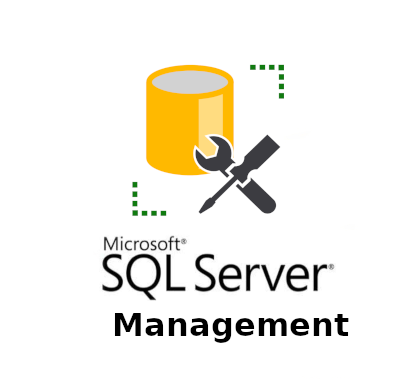
\includegraphics[width=6cm]{Figures/sqlmanagementstudio.png}
        \caption{Microsoft SQL Server management studio logo}
    %\label{fig:my_label} %Optional (If you want to reference the figure in later chapters)
\end{figure}


\textbf{Visual Studio} : est un IDE complet développé par Microsoft, utilisé pour développer des applications informatiques, des sites web, des services web, des applications mobiles et bien plus encore. Il prend en charge plusieurs langages de programmation, notamment C\#, VB.NET, C++, Python, et d'autres. Visual Studio offre des outils de développement, de débogage et de test intégrés, ce qui en fait un choix populaire parmi les développeurs pour la création d'applications de haute qualité.
\\
\begin{figure}[H] 
    \centering
    
\includegraphics[width=4cm]{Figures/Visual-Studio-logo.png}
        \caption{Microsoft Visual studio logo}
    %\label{fig:my_label} %Optional (If you want to reference the figure in later chapters)
\end{figure}




\textbf{Visual Studio Code} : est un éditeur de code source léger mais puissant développé par Microsoft. Il offre aux développeurs un riche ensemble de fonctionnalités pour éditer, déboguer et gérer du code dans divers langages de programmation et plateformes. Nous l'avons largement utilisé pour le développement de nouvelles fonctionnalités dans Fawri Form. Son interface intuitive, son intégration Git intégrée et sa vaste bibliothèque d'extensions en ont fait le choix idéal pour notre workflow de développement. Grâce à VS Code, nous avons pu écrire, déboguer et tester du code de manière efficace, collaborer avec les membres de l'équipe en utilisant le contrôle de version et personnaliser notre environnement de développement en fonction de nos besoins spécifiques.
\\
\begin{figure}[H] 
    \centering
    
\includegraphics[width=3cm]{Figures/vsclogo.png}
        \caption{Microsoft Visual studio code logo}
    %\label{fig:my_label} %Optional (If you want to reference the figure in later chapters)
\end{figure}




\textbf{Git} : est un système de gestion de version largement utilisé dans le développement logiciel pour suivre les modifications apportées au code source durant la phase de développement. Il permet aux programmeurs de travailler simultanément sur un projet en suivant les différentes versions des documents ainsi que les modifications effectuées par plusieurs personnes. Git fonctionne dans l'environnement local d'un développeur, permettant de travailler en mode hors ligne et de faire des commits dans le référentiel local. Il offre également de solides fonctionnalités de branchement et de fusion, permettant aux utilisateurs de créer des branches pour les nouvelles fonctionnalités ou les corrections, qui peuvent ensuite être facilement fusionnées dans le flux principal de code. Git est capable de suivre les changements de code et sa structure de branchement permet la gestion des versions, la gestion du temps et le travail distribué. De plus, il fonctionne en conjonction avec de nombreux hébergeurs tels qu'Azure DevOps, GitHub, GitLab et Bitbucket pour le dépôt de code, le partage de code et le suivi de projet.
\\
\begin{figure}[H] 
    \centering
    
\includegraphics[width=8cm]{Figures/gitlogo.jpg}
        \caption{Git logo}
    %\label{fig:my_label} %Optional (If you want to reference the figure in later chapters)
\end{figure}



\section{Environnement de Test}


\textbf{xUnit.net} : Pour la réalisation des tests unitaires, nous avons opté pour le Framework xUnit.net. Il s'agit d'un outil open source dédié aux tests unitaires dans le cadre du .NET Framework et bénéficiant d'un fort soutien de la communauté. Conçu par l'inventeur original de NUnit v2, xUnit.net constitue la technologie de pointe en matière de tests unitaires pour les langages tels que C\#, F\#, VB.NET et autres langages .NET.
\\
\begin{figure}[H] 
    \centering
    
\includegraphics[width=6cm]{Figures/xunitlogo.png}
        \caption{xUnit.net logo}
    %\label{fig:my_label} %Optional (If you want to reference the figure in later chapters)
\end{figure}


\textbf{Swagger} : est un ensemble d'outils open source permettant de concevoir, de construire, de documenter et de consommer des services web RESTful. Il offre une interface conviviale pour décrire la structure des API REST, ainsi que la possibilité de générer automatiquement une documentation interactive à partir de ces descriptions. Swagger simplifie le processus de développement et de maintenance des API en fournissant une manière standardisée de définir et de partager les spécifications des API.
\\
\begin{figure}[H] 
    \centering
    
\includegraphics[width=6cm]{Figures/swaggerlogo.png}
        \caption{Swagger logo}
    %\label{fig:my_label} %Optional (If you want to reference the figure in later chapters)
\end{figure}



\section{Outils de conception et modélisation}


Dans ce projet, nous avons utilisé plusieurs outils pour la conception et la modélisation des différents aspects du système. Parmi ces outils, nous avons principalement utilisé UML (Unified Modeling Language). UML est un langage de modélisation visuelle standardisé, utilisé pour représenter les différents composants et interactions d'un système logiciel. Il permet de créer des diagrammes de cas d'utilisation, de classes, de séquence et bien d'autres, facilitant ainsi la compréhension et la conception du système.
\\
\begin{figure}[H] 
    \centering
    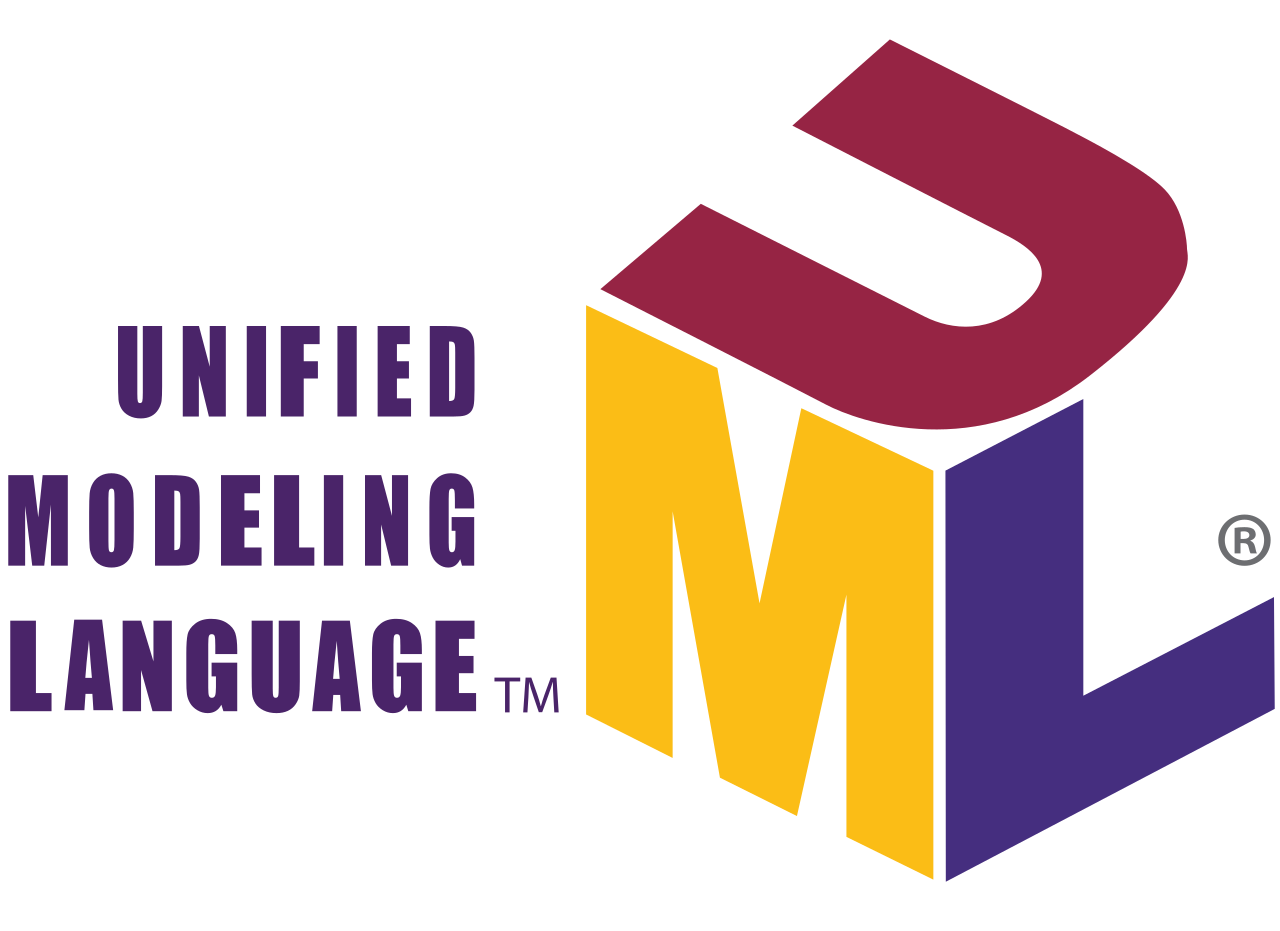
\includegraphics[width=6cm]{Figures/UML_logo.svg.png}
        \caption{UML logo}
    %\label{fig:my_label} %Optional (If you want to reference the figure in later chapters)
\end{figure}

En plus de UML, nous avons également employé Figma, une plateforme de conception collaborative, pour créer des maquettes et des prototypes interactifs de l'interface utilisateur. Figma nous a permis de visualiser et de tester l'aspect visuel et l'ergonomie de l'application avant son développement.
\\
\begin{figure}[H] 
    \centering
    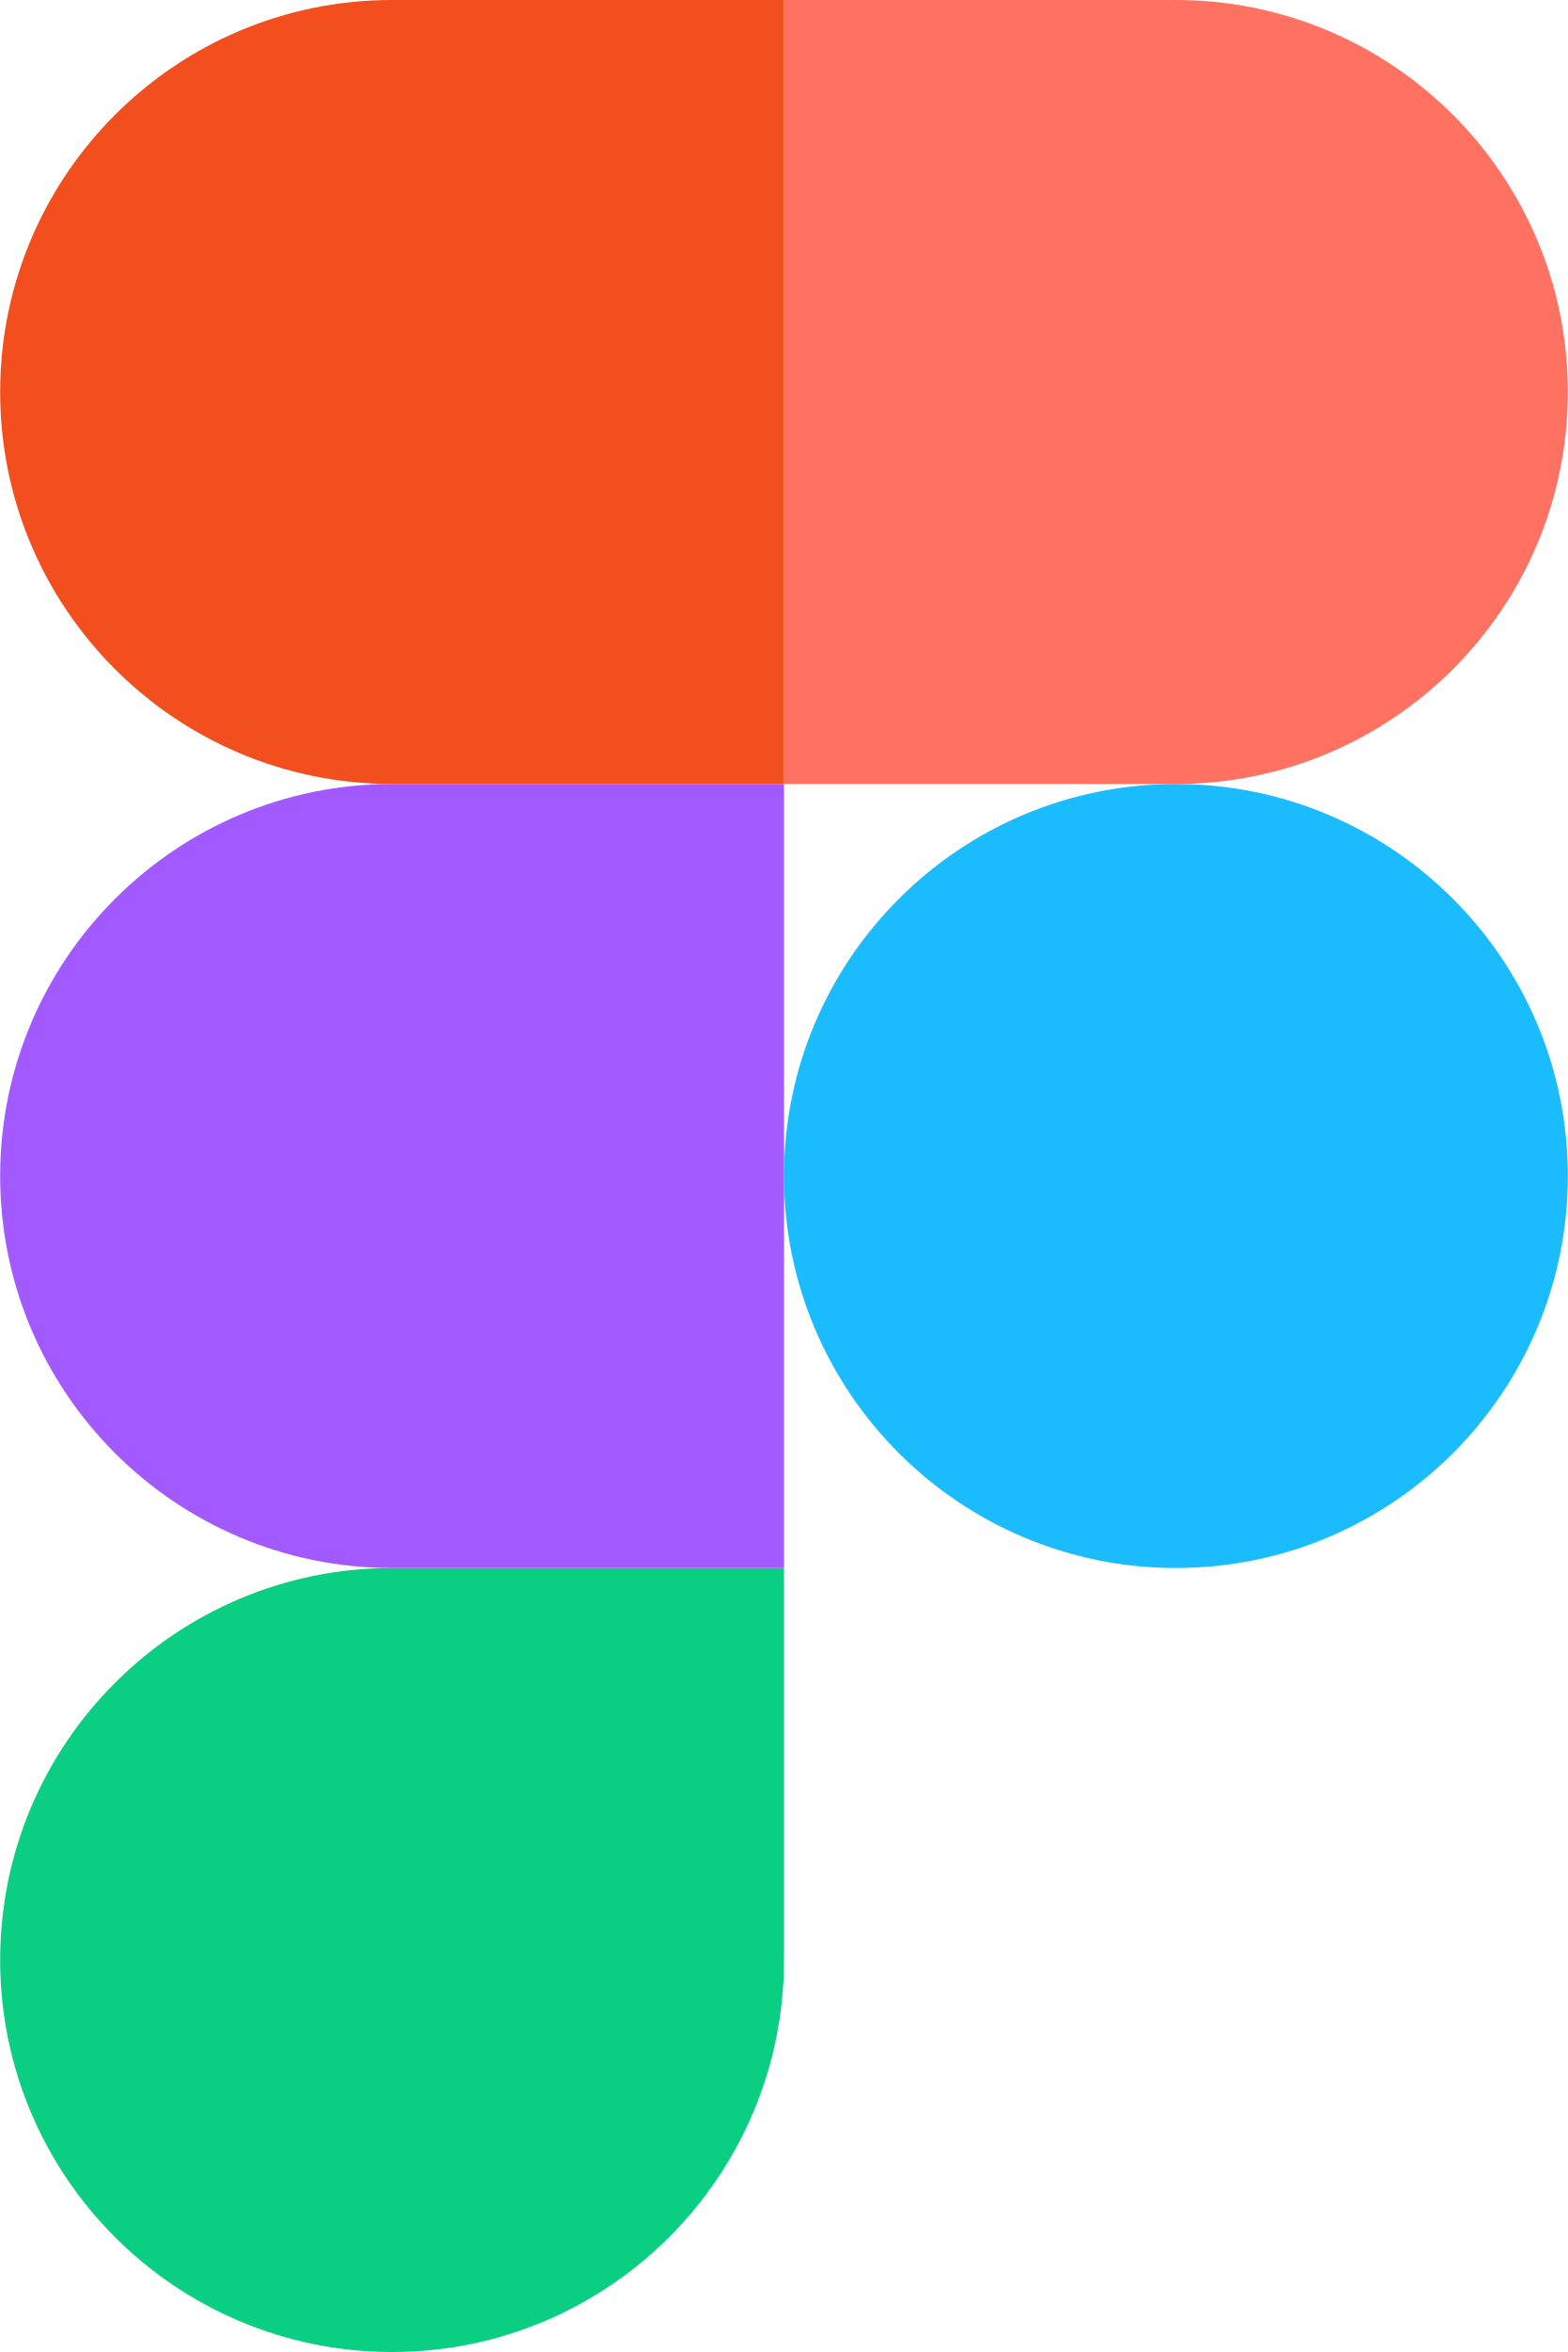
\includegraphics[width=3cm]{Figures/figma logo.png}
        \caption{Figma logo}
    %\label{fig:my_label} %Optional (If you want to reference the figure in later chapters)
\end{figure}

En combinant ces outils, nous avons pu élaborer des représentations visuelles précises et détaillées de notre système, facilitant ainsi la communication et la collaboration entre les membres de l'équipe de développement.




\section{Concepts et Méthodologie}

Cette section offre une analyse approfondie des principes de conception logicielle et des méthodologies de développement les plus répandues. Nous y mettons en avant les meilleures pratiques de développement ainsi que les concepts fondamentaux qui guident la création de notre système.

\subsection{Test Driven Development}


\begin{figure}[H] 
    \centering
    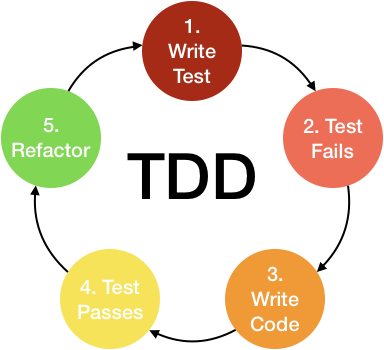
\includegraphics[width=6cm]{Figures/TDD.png}
        \caption{Cycle TDD}
    %\label{fig:my_label} %Optional (If you want to reference the figure in later chapters)
\end{figure}



Le Test-Driven Development (TDD), ou développement piloté par les tests, se démarque des approches traditionnelles par son approche inversée. Contrairement à la rédaction du code en premier lieu, le TDD met l'accent sur la création de tests automatisés qui spécifient le comportement attendu de chaque fonctionnalité. Ce processus itératif et incrémental se divise en trois étapes clés : 
\begin{enumerate} 

    \item \textbf{Rédiger un test qui échoue} : Le développeur commence par définir un test automatisé qui reflète le comportement souhaité de la fonctionnalité à implémenter. Ce test échoue initialement, car le code n'existe pas encore.

    \item \textbf{Écrire le code pour passer le test} : L'objectif est de développer le code minimal requis pour que le test automatisé précédemment créé réussisse. Il ne s'agit pas de produire un code parfait à ce stade, mais plutôt de répondre aux exigences essentielles du test.

    \item \textbf{Refactoriser le code} : Une fois le test réussi, le code est refactorisé pour améliorer sa structure, sa lisibilité et sa maintenabilité. Cette étape garantit que le code reste propre et évolutif, sans affecter le bon fonctionnement des tests.
\end{enumerate}

L'approche TDD offre de nombreux avantages :
\begin{itemize}
    \item \textbf{Amélioration de la qualité du code} : Les tests automatisés contraignent le développeur à écrire un code robuste et exempt de bugs.

    \item \textbf{Réduction des défauts} : En détectant les erreurs dès les premières étapes du développement, le TDD minimise le nombre de bugs à corriger ultérieurement.

    \item \textbf{Compréhension accrue des exigences} : Le processus de création de tests oblige le développeur à analyser et à clarifier les exigences fonctionnelles, menant à une meilleure compréhension du projet.
\end{itemize}

Ce projet est mis en place en respectant cette approche. Autrement dit, pour chaque intention obtenue à propos d’une fonctionnalité, un test est rédigé. Celui-ci échoue au début, mais après l’implémentation initiale de la fonctionnalité, il passe. Puis reste d’effectuer des refactorisations afin d’achever la fonctionnalité.



\subsection{Domain-Driven Design (DDD)}

Dans cette section, nous aborderons le Domain-Driven Design (DDD), une méthodologie de développement logiciel axée sur une compréhension approfondie et une modélisation précise du domaine métier d'une application. Contrairement à une approche uniquement technique, le DDD vise à harmoniser le code et la structure logicielle avec les concepts et le langage spécifiques au domaine concerné. Cette intégration permet aux développeurs de mieux répondre aux besoins et exigences propres au domaine, favorisant ainsi la création d'un code plus souple, modulaire et facilement maintenable. 




Les principes clés du Domain-Driven Design (DDD) comprennent :
\begin{itemize}
    \item \textbf{Prioriser le domaine métier} : Le DDD positionne le domaine métier comme pilier central de la conception logicielle. Il incite les développeurs à s'immerger dans le domaine d'activité concerné, en collaborant étroitement avec les experts métier et en adoptant un langage commun pour décrire les concepts et processus métier.

    \item \textbf{Modélisation du domaine} : Au cœur de la démarche DDD se trouve la création d'un modèle du domaine métier. Ce modèle, tel un miroir du domaine réel, représente ses entités, agrégats, valeurs-objets, services et règles métier. Il sert à capturer les concepts clés du domaine et les interactions qui les lient, offrant une vision claire et structurée du système.

    \item \textbf{Bounded Contexts (Contextes limités)} : Le domaine métier peut être fragmenté en plusieurs contextes délimités, chacun possédant sa propre sémantique et ses règles métier spécifiques. Ces contextes délimités agissent comme des modules autonomes, favorisant la gestion de la complexité en délimitant les interactions entre les différentes parties du système.

    \item \textbf{Ubiquitous Language (Langage omniprésent)} : Le DDD met l'accent sur l'utilisation d'un langage commun, appelé "langage omniprésent", qui est partagé entre les experts métier et les développeurs. Ce langage permet de réduire les ambiguïtés et d'assurer une compréhension commune des concepts et des termes utilisés dans le domaine.

    \item \textbf{Agrégats} : Les agrégats représentent des ensembles d'objets étroitement liés, considérés comme une unité cohérente dans le modèle du domaine. Ils délimitent les transactions et assurent la cohérence des données.

    \item \textbf{Entités et Objets Valeur} : Les entités sont des objets ayant une identité distincte et se définissent par leurs attributs et comportements. Elles représentent des concepts avec des identités uniques et des cycles de vie propres au sein du domaine. En revanche, les objets valeur sont des objets dépourvus d'identité distincte et se définissent uniquement par leurs attributs. Ils représentent des valeurs ou des caractéristiques immuables au sein du domaine. Ensemble, les entités et les objets valeur constituent les éléments fondamentaux du modèle de domaine, chacun jouant un rôle spécifique pour capturer les nuances du domaine métier.
\end{itemize}

En adoptant les principes du DDD, nous pouvons concevoir des solutions logicielles mieux adaptées aux environnements complexes et aux applications de grande envergure.

Il existe quatre couches fondamentales dans une solution basée sur le Domain Driven Design (DDD).

\begin{figure}[H] 
    \centering
    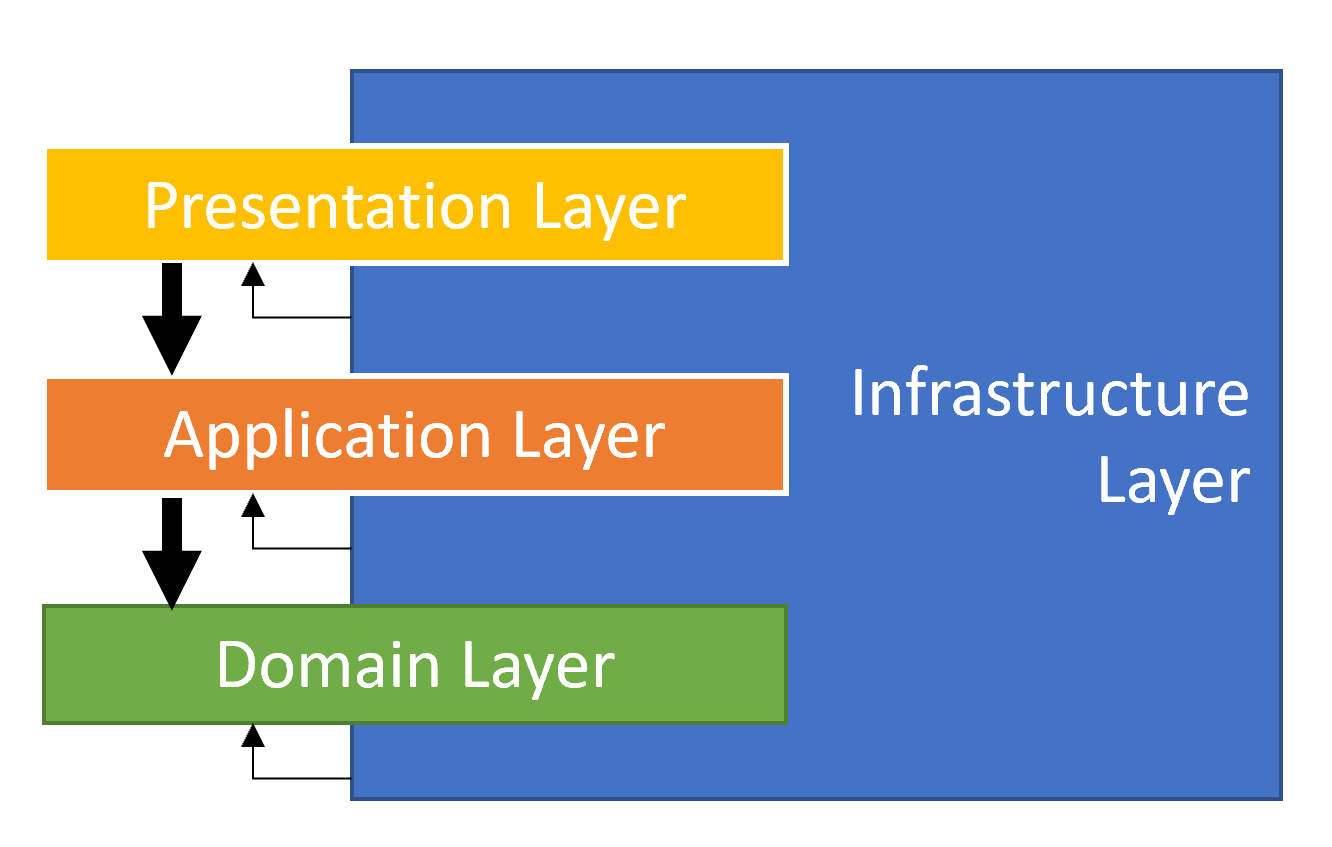
\includegraphics[width=9cm]{Figures/dddl.png}
        \caption{Les couches DDD}
    %\label{fig:my_label} %Optional (If you want to reference the figure in later chapters)
\end{figure}


\begin{itemize}
    \item \textbf{Couche Domaine (Domain Layer) :}
        \begin{itemize}
            \item Contient la logique métier centrale et indépendante des cas d'utilisation spécifiques.
            \item Implémente les règles, les entités, les valeurs objets et les agrégats qui définissent le cœur du système.
        \end{itemize}




    \item \textbf{Couche Application (Application Layer) :}
        \begin{itemize}
            \item Gère les cas d'utilisation de l'application en se basant sur les concepts du domaine.
            \item Ordonne et coordonne les opérations de domaine pour satisfaire les requêtes de l'utilisateur.
            \item Peut être considérée comme la couche qui orchestre les interactions utilisateur sur l'interface utilisateur (UI).
        \end{itemize}







    \item \textbf{Couche Présentation (Presentation Layer):}
        \begin{itemize}
            \item Comprend les éléments de l'interface utilisateur (UI), tels que les pages et les composants.
            \item Responsable de l'affichage des informations et de la gestion des interactions utilisateur.
        \end{itemize}






    \item \textbf{Couche Infrastructure (Infrastructure Layer) :}
        \begin{itemize}
            \item Supporte les autres couches en fournissant les abstractions et les intégrations nécessaires avec les bibliothèques tierces et les systèmes externes.
            \item Gère les aspects techniques tels que la persistance des données, les services externes, les messages et les événements.
        \end{itemize}
    
\end{itemize}



\subsection{Développement basé sur le tronc (Trunk-Based Development)}

\hspace{\parindent} Pour notre projet de fin d’études, nous avons adopté le développement basé sur le tronc (Trunk-Based Development, TBD) comme méthodologie de gestion de code source. Le TBD nous a permis d'intégrer fréquemment des modifications dans une seule branche principale, appelée "tronc" ou "master", ce qui a facilité une intégration continue et rapide, réduit les risques de conflits de fusion et soutenu une livraison continue efficace.

% \begin{figure}[H] 
%     \centering
%     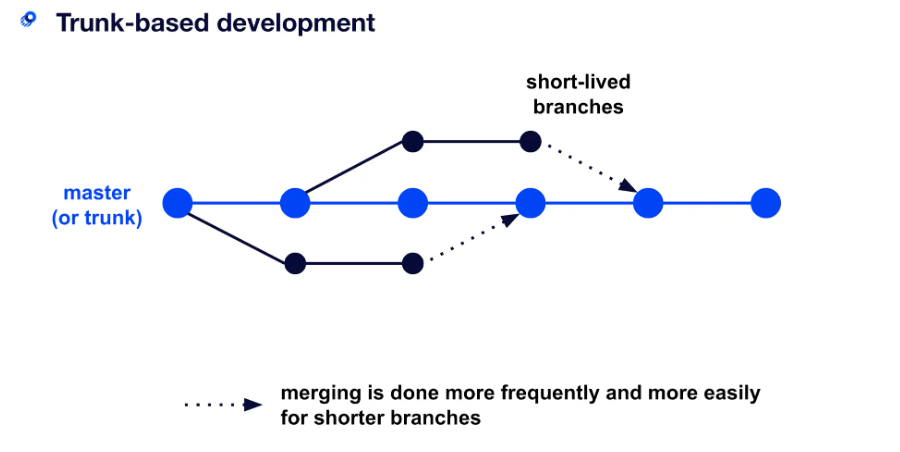
\includegraphics[width=9cm]{Figures/tbd.png}
%         \caption{Gestion des branches selon TBD}
%     %\label{fig:my_label} %Optional (If you want to reference the figure in later chapters)
% \end{figure}

\textbf{-----------------------------------------------INSERT IMAGE tbd-----------
----------------------------------------}

L'approche TBD a plusieurs avantages:
\begin{itemize}

    \item \textbf{Intégration Continue} : En intégrant notre code régulièrement dans le tronc, nous avons pu détecter et résoudre précocement les conflits et les problèmes d'intégration.
    
    \item \textbf{Livraison Continue} : Cette approche a parfaitement complété notre pratique de livraison continue, nous permettant de déployer des mises à jour fréquentes et fiables.

    \item \textbf{Réduction des Conflits} : En évitant les branches de longue durée, nous avons minimisé les conflits de fusion, simplifiant ainsi notre processus de développement.

    \item \textbf{Collaboration Accrue} : En travaillant tous sur la même branche, nous avons favorisé une meilleure collaboration et une communication plus fluide au sein de notre équipe.
    
\end{itemize}





\subsection{Multitenancy : Une Architecture Efficace et Évolutive pour les Applications SaaS}



\hspace{\parindent}La \textit{multitenancy} est une approche dans laquelle une seule instance d'une application logicielle sert plusieurs organisations distinctes, appelées tenants. Chaque tenant opère comme s'il disposait de sa propre instance dédiée, avec des données et des configurations spécifiques, mais tous partagent la même infrastructure sous-jacente. Ses principes de base sont :

\begin{itemize}
    \item Isolation des Données : Les données de chaque tenant sont isolées pour garantir la confidentialité et la sécurité.

    \item Personnalisation : Chaque tenant peut personnaliser certains aspects de l'application (comme l'interface utilisateur et les configurations).

    \item Gestion des Ressources : Les ressources informatiques sont partagées entre les tenants, ce qui permet une utilisation plus efficace des ressources.
    
\end{itemize}


La \textit{multitenancy} présente plusieurs avantages, notamment dans le contexte des applications cloud et des services logiciels (SaaS). Voici quelques-uns des principaux avantages :

\begin{itemize}
    \item Efficacité des Coûts : Réduit les coûts d'infrastructure en partageant les mêmes ressources matérielles et logicielles entre plusieurs tenants.

    \item Facilité de Maintenance : Simplifie les mises à jour et la maintenance puisque les modifications apportées à une seule instance de l'application sont appliquées à tous les tenants.

    \item Évolutivité : Permet une montée en charge plus aisée en répartissant les coûts de développement et de maintenance sur plusieurs utilisateurs.

    \item Gestion Simplifiée : Facilite la gestion globale de l'application grâce à une seule base de code et une seule infrastructure.

    
\end{itemize}


\begin{figure}[H] 
    \centering
    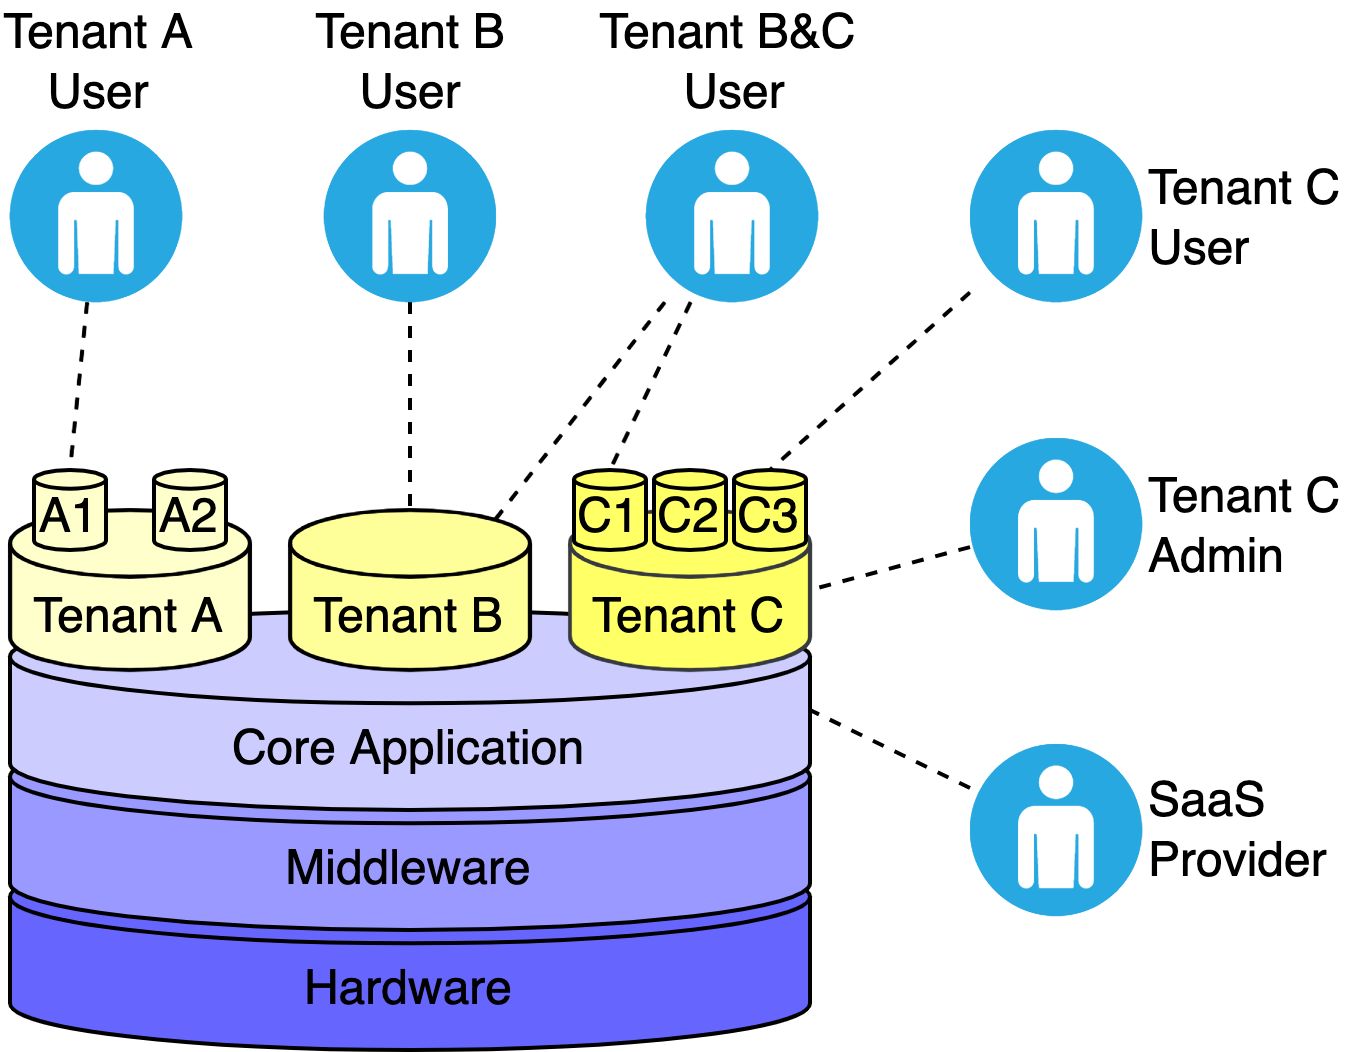
\includegraphics[width=9cm]{Figures/multytenancy.png}
        \caption{Le principe de la multitenancy}
    %\label{fig:my_label} %Optional (If you want to reference the figure in later chapters)
\end{figure}

\section{Architecture de la solution}

\subsection{Architecture de la solution Fawri-CMS suivant le DDD}

\hspace{\parindent}La figure suivante illustre un flux de demande typique pour une application web développée selon le DDD:


\begin{figure}[H] 
    \centering
    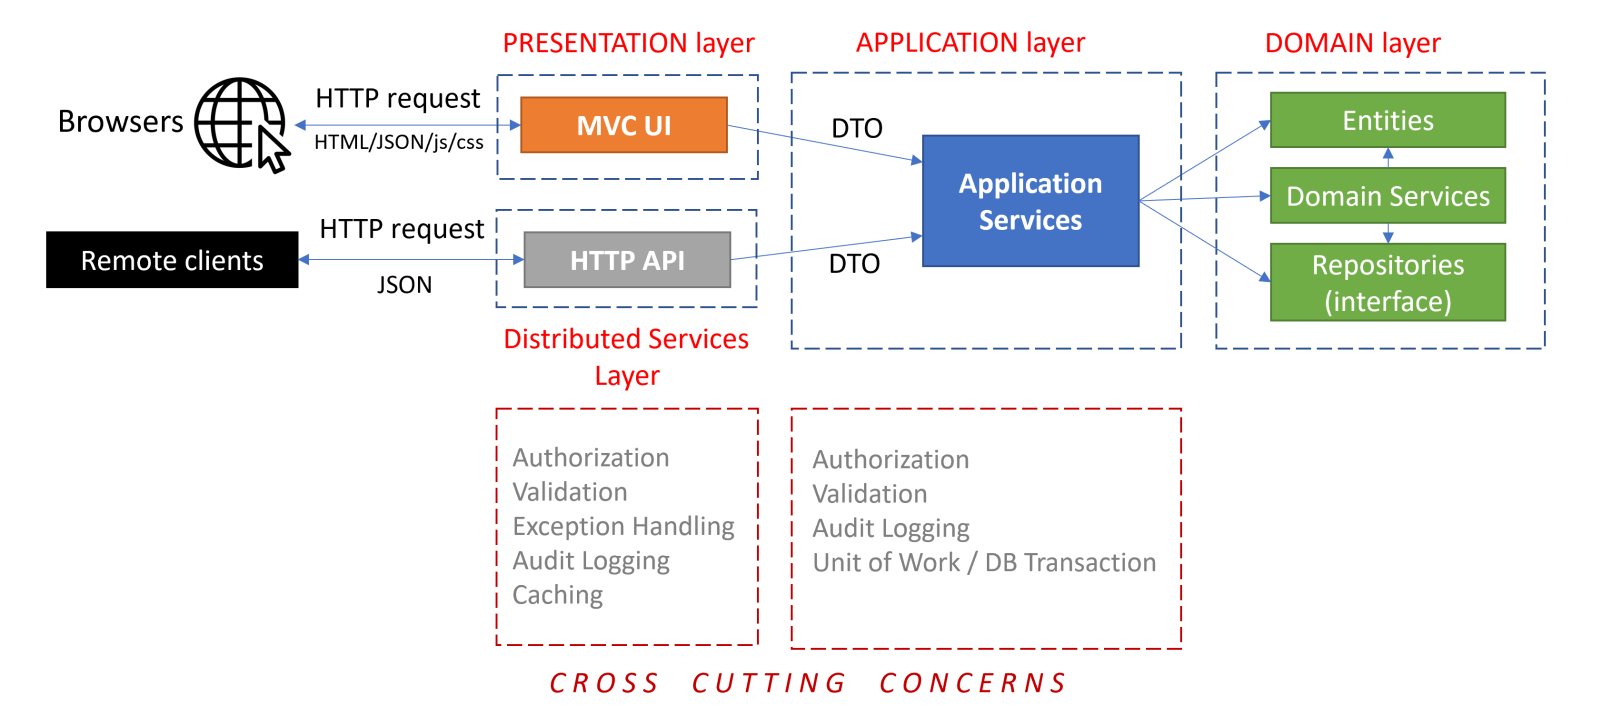
\includegraphics[width=17cm]{Figures/DDD flow.png}
        \caption{L'architecture de la solution suivant DDD }
    %\label{fig:my_label} %Optional (If you want to reference the figure in later chapters)
\end{figure}


\begin{enumerate}
    \item Le navigateur de l'utilisateur envoie une requête HTTP au serveur web ;

\item Le serveur web reçoit la requête et la transmet à l'application ;

\item Dans la couche de présentation, le contrôleur ou le gestionnaire de requêtes traite la demande et Interagit avec les autres couches de l'application ;

\item Le contrôleur ou le gestionnaire de requêtes interroge la couche d'application pour obtenir les données nécessaires pour répondre à la demande ;
\item. Dans la couche d'application, les services applicatifs coordonnent l'exécution des cas d'utilisation métier ;

\item Les services applicatifs utilisent la couche de domaine pour accéder aux entités, aux agrégats et aux règles métier ;

\item La couche de domaine encapsule la logique métier et interagit avec la couche d'infrastructure pour récupérer ou persister les données ;

\item La couche d'infrastructure communique avec le système de persistance (base de données, API externe, etc.) pour récupérer ou enregistrer les données ;

\item Une fois que les données ont été récupérées, la couche d'infrastructure les renvoie à la couche d'application ;

\item La couche d'application agrège les données et les prépare pour être renvoyées à la couche de présentation ;

\item La couche de présentation utilise les données reçues pour générer une réponse appropriée à la requête initiale ;
\item La réponse est renvoyée au serveur web qui la transmet ensuite au navigateur de l'utilisateur ;

\item Le navigateur de l'utilisateur affiche la réponse dans l'interface utilisateur.
\end{enumerate}


Ce flux de demande suit les principes du DDD, où la logique métier est encapsulé dans la couche de domaine et la couche d'application coordonne l'exécution des cas d'utilisation. Les différentes couches travaillent ensemble pour fournir une réponse aux demandes des utilisateurs de l'application web.

\subsection{Architecture technique suivant le Template d’ABP}

\hspace{\parindent}Nous avons démarré le projet en utilisant ABP CLI pour générer la structure initiale. Ensuite, nous avons intégré le code dans un référentiel de versionnement hébergé sur Azure DevOps, ce qui nous permet de collaborer efficacement, de suivre les modifications du code et d'automatiser les processus de développement tels que l'intégration continue et la livraison continue (CI/CD).


Le projet est structuré en deux répertoires principaux : « src » et « test ». L'architecture de la solution est illustrée dans la figure suivante.



\begin{figure}[H] 
    \centering
    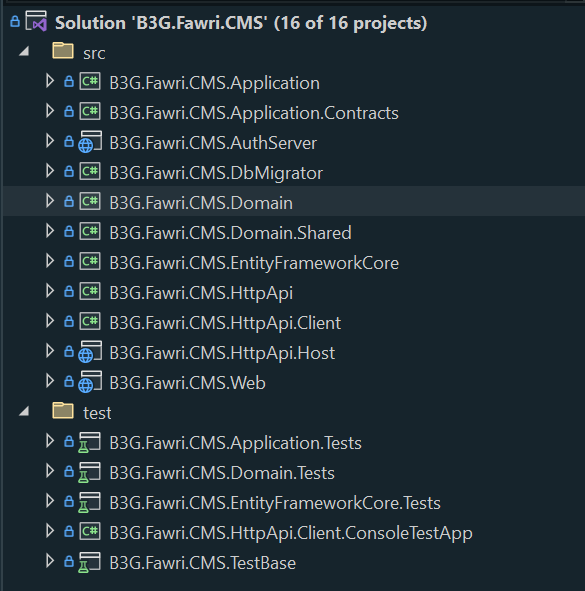
\includegraphics[width=9cm]{Figures/src test.PNG}
        \caption{Structure du projet Fawri-CMS}
    %\label{fig:my_label} %Optional (If you want to reference the figure in later chapters)
\end{figure}


Chaque couche de l'architecture suit le principe SOLID (Single Responsibility), ce qui signifie qu'elle possède une seule responsabilité et un seul objectif de fonctionnement. ABP Framework, basé sur une architecture en couches, favorise une séparation claire des responsabilités et une modularité.

\begin{itemize}
    \item \textbf{Couche de présentation (Presentation Layer)} :

Responsable de l'interface utilisateur de l'application, cette couche peut se présenter sous différentes formes telles qu'une application web, mobile, une API REST ou une interface utilisateur de bureau. Elle communique avec la couche d'application pour afficher les données et gérer les interactions utilisateur.\\

\begin{figure}[H] 
    \centering
    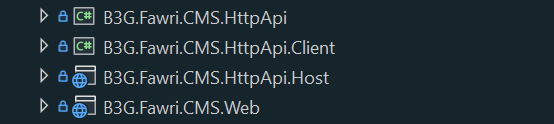
\includegraphics[width=9cm]{Figures/presentation layer.PNG}
        \caption{Couche Presentation}
    %\label{fig:my_label} %Optional (If you want to reference the figure in later chapters)
\end{figure}

    \item \textbf{Couche d'application (Application Layer)} :

    Cette couche gère la logique métier de l'application. Elle contient les services d'application qui encapsulent les cas d'utilisation et les règles métier spécifiques. Les services d'application agissent comme une interface entre les couches supérieures et inférieures, orchestrant l'exécution des opérations de l'application.



\begin{figure}[H] 
    \centering
    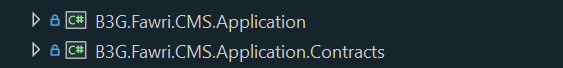
\includegraphics[width=9cm]{Figures/application layer.PNG}
        \caption{Couche Application}
    %\label{fig:my_label} %Optional (If you want to reference the figure in later chapters)
\end{figure}





    \item \textbf{Couche d'infrastructure (Infrastructure Layer)} :
    Fournit des services et des implémentations techniques pour soutenir les fonctionnalités de l'application. Elle comprend des classes utilitaires, des gestionnaires de persistance, des implémentations de fournisseurs de services tiers, des services d'authentification, des services de messagerie.

\begin{figure}[H] 
    \centering
    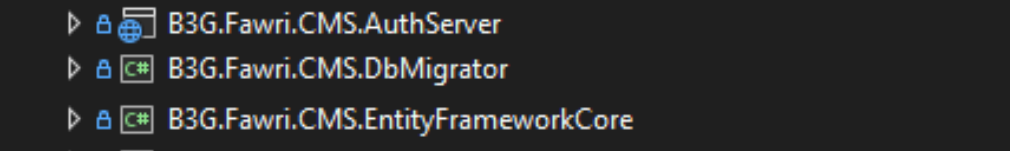
\includegraphics[width=9cm]{Figures/infra layer.PNG}
        \caption{Couche Infrastructure}
    %\label{fig:my_label} %Optional (If you want to reference the figure in later chapters)
\end{figure}






\item \textbf{Couche de domaine (Domain Layer)} :

Représente le cœur de l'application. Elle définit les entités métier, les agrégats, les valeurs d'objet et les règles métier. Cette couche est indépendante de l'infrastructure et peut être réutilisée dans différents contextes d'application.

    \begin{figure}[H] 
    \centering
    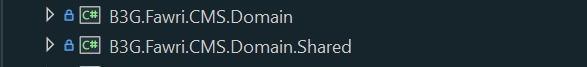
\includegraphics[width=9cm]{Figures/domain layer.PNG}
        \caption{Couche Domain}
    %\label{fig:my_label} %Optional (If you want to reference the figure in later chapters)
\end{figure}

\end{itemize}



En plus des couches de DDD représentées par les projets situés dans le dossier src, nous avons également le dossier test (généré par ABP). Ce dossier contient les projets de tests, où nous écrivons et exécutons les tests pour notre projet. La capture d'écran fournie montre la structure du dossier test, avec plusieurs sous-projets :
\begin{figure}[H] 
    \centering
    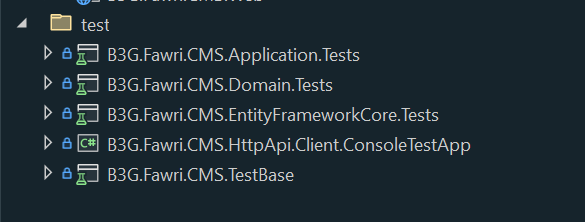
\includegraphics[width=9cm]{Figures/test folder.PNG}
        \caption{La structure du dossier \textit{test}}
    %\label{fig:my_label} %Optional (If you want to reference the figure in later chapters)
\end{figure}








\newpage
\section*{Conclusion}

\hspace{\parindent}Après avoir pris le temps d'explorer en profondeur l'architecture technique adoptée pour notre système à venir, ainsi que les différents outils et frameworks qui seront indispensables à sa réalisation, le prochain chapitre se penchera sur les étapes suivies pour donner vie à ce projet ambitieux.

\pagebreak